\documentclass{article}
\usepackage{neurips_2026}
\usepackage[utf8]{inputenc}
\usepackage[T1]{fontenc}
\usepackage{hyperref}
\usepackage{url}
\usepackage{booktabs}
\usepackage{amsfonts,amsmath,amssymb}
\usepackage{nicefrac}
\usepackage{microtype}
\usepackage{xcolor}
\usepackage{graphicx}
\newcommand{\NAArenadropalpha}{10.5\%}
\newcommand{\NAArenadropkappa}{0.148}
\newcommand{\NAArenadropphi}{0.51}
\newcommand{\NAArenadropz}{9.62}
\newcommand{\NAArenainsertalpha}{8.3\%}
\newcommand{\NAArenainsertkappa}{0.138}
\newcommand{\NAArenainsertphi}{0.44}
\newcommand{\NAArenainsertz}{9.62}
\newcommand{\NAArenarelabelalpha}{4.2\%}
\newcommand{\NAArenarelabelkappa}{0.071}
\newcommand{\NAArenarelabelphi}{0.23}
\newcommand{\NAArenarelabelz}{9.62}
\newcommand{\NAMTGdropalpha}{16.7\%}
\newcommand{\NAMTGdropkappa}{0.157}
\newcommand{\NAMTGdropphi}{0.54}
\newcommand{\NAMTGdropz}{13.68}
\newcommand{\NAMTGinsertalpha}{11.0\%}
\newcommand{\NAMTGinsertkappa}{0.112}
\newcommand{\NAMTGinsertphi}{0.39}
\newcommand{\NAMTGinsertz}{13.68}
\newcommand{\NAMTGrelabelalpha}{6.5\%}
\newcommand{\NAMTGrelabelkappa}{0.063}
\newcommand{\NAMTGrelabelphi}{0.22}
\newcommand{\NAMTGrelabelz}{13.68}
\newcommand{\NAMTHdropalpha}{10.2\%}
\newcommand{\NAMTHdropkappa}{0.163}
\newcommand{\NAMTHdropphi}{0.56}
\newcommand{\NAMTHdropz}{8.70}
\newcommand{\NAMTHinsertalpha}{8.0\%}
\newcommand{\NAMTHinsertkappa}{0.130}
\newcommand{\NAMTHinsertphi}{0.45}
\newcommand{\NAMTHinsertz}{8.70}
\newcommand{\NAMTHrelabelalpha}{4.4\%}
\newcommand{\NAMTHrelabelkappa}{0.072}
\newcommand{\NAMTHrelabelphi}{0.24}
\newcommand{\NAMTHrelabelz}{8.70}
\newcommand{\NJatheneadjsig}{11\%}
\newcommand{\NJathenekappa}{0.054}
\newcommand{\NJathenephi}{0.27}
\newcommand{\NJathenetau}{0.79}
\newcommand{\NJathenetie}{4\%}
\newcommand{\NJathenez}{9.0}
\newcommand{\NJhumanadjsig}{6\%}
\newcommand{\NJhumankappa}{0.064}
\newcommand{\NJhumannotiesadjsig}{3\%}
\newcommand{\NJhumannotieskappa}{0.057}
\newcommand{\NJhumannotiesphi}{0.28}
\newcommand{\NJhumannotiestau}{0.98}
\newcommand{\NJhumannotiestie}{0\%}
\newcommand{\NJhumannotiesz}{5.4}
\newcommand{\NJhumanphi}{0.24}
\newcommand{\NJhumantau}{1.00}
\newcommand{\NJhumantie}{31\%}
\newcommand{\NJhumanz}{5.7}
\newcommand{\NJllamaadjsig}{10\%}
\newcommand{\NJllamakappa}{0.055}
\newcommand{\NJllamaphi}{0.27}
\newcommand{\NJllamatau}{0.71}
\newcommand{\NJllamatie}{2\%}
\newcommand{\NJllamaz}{8.2}
\newcommand{\NJmistraladjsig}{8\%}
\newcommand{\NJmistralkappa}{0.060}
\newcommand{\NJmistralphi}{0.29}
\newcommand{\NJmistraltau}{0.69}
\newcommand{\NJmistraltie}{1\%}
\newcommand{\NJmistralz}{6.4}
\newcommand{\Nadjalphaarenadrop}{0.009\%}
\newcommand{\Nadjalphaarenainsert}{0.009\%}
\newcommand{\Nadjalphaarenarelabel}{0.005\%}
\newcommand{\NadjalphamtgptFourdrop}{5.96\%}
\newcommand{\NadjalphamtgptFourinsert}{5.04\%}
\newcommand{\NadjalphamtgptFourrelabel}{2.54\%}
\newcommand{\Nadjalphamthumandrop}{4.20\%}
\newcommand{\Nadjalphamthumaninsert}{3.99\%}
\newcommand{\Nadjalphamthumanrelabel}{2.00\%}
\newcommand{\Nadjalphanbadrop}{0.18\%}
\newcommand{\Nadjalphanbainsert}{0.17\%}
\newcommand{\Nadjalphanbarelabel}{0.11\%}
\newcommand{\NadjkarenaNewdrop}{13}
\newcommand{\NadjkarenaNewinsert}{11}
\newcommand{\NadjkarenaNewrelabel}{6}
\newcommand{\Nadjkarenadrop}{5}
\newcommand{\Nadjkarenainsert}{5}
\newcommand{\Nadjkarenarelabel}{3}
\newcommand{\NadjkmtgptFourdrop}{143}
\newcommand{\NadjkmtgptFourinsert}{121}
\newcommand{\NadjkmtgptFourrelabel}{61}
\newcommand{\Nadjkmthumandrop}{141}
\newcommand{\Nadjkmthumaninsert}{134}
\newcommand{\Nadjkmthumanrelabel}{67}
\newcommand{\Nadjknbadrop}{2}
\newcommand{\Nadjknbainsert}{2}
\newcommand{\Nadjknbarelabel}{1}
\newcommand{\Nadjsigarena}{6\%}
\newcommand{\NadjsigarenaOneFourZerok}{10\%}
\newcommand{\NadjsigarenaNew}{10\%}
\newcommand{\NadjsigmtgptFour}{100\%}
\newcommand{\Nadjsigmthuman}{80\%}
\newcommand{\Nadjsignba}{1\%}
\newcommand{\Nadjzarenadrop}{0.24}
\newcommand{\Nadjzarenainsert}{0.24}
\newcommand{\Nadjzarenarelabel}{0.24}
\newcommand{\NadjzmtgptFourdrop}{8.71}
\newcommand{\NadjzmtgptFourinsert}{8.71}
\newcommand{\NadjzmtgptFourrelabel}{8.71}
\newcommand{\Nadjzmthumandrop}{8.06}
\newcommand{\Nadjzmthumaninsert}{8.06}
\newcommand{\Nadjzmthumanrelabel}{8.06}
\newcommand{\Nadjznbadrop}{0.24}
\newcommand{\Nadjznbainsert}{0.24}
\newcommand{\Nadjznbarelabel}{0.24}
\newcommand{\NarenaNewM}{53}
\newcommand{\NarenaNewMulti}{25\%}
\newcommand{\NarenaNewN}{135{,}634}
\newcommand{\NarenaNewSessions}{115{,}372}
\newcommand{\Narenasixn}{1367}
\newcommand{\Narenatopa}{gpt-4-1106-preview}
\newcommand{\Narenatopb}{gpt-4-0125-preview}
\newcommand{\Narenatopgap}{0.7}
\newcommand{\Narenatopz}{0.07}
\newcommand{\Nbasepairs}{503}
\newcommand{\Nbaserandmax}{5.4}
\newcommand{\Nbaserandmin}{1.5}
\newcommand{\Nbasetoucheq}{93\%}
\newcommand{\Ncensfrac}{0.003\%}
\newcommand{\Nclnq}{80}
\newcommand{\Nclpairsmtg}{15}
\newcommand{\Nclpairsmth}{14}
\newcommand{\Nclqmtg}{68\%}
\newcommand{\Nclqmth}{68\%}
\newcommand{\Nclratiomtg}{5.9}
\newcommand{\Nclratiomth}{5.9}
\newcommand{\Ncltopmtg}{30}
\newcommand{\Ncltopmth}{11}
\newcommand{\Nclvmtg}{11.6\%}
\newcommand{\Nclvmth}{11.6\%}
\newcommand{\Nfracmaxratio}{1.027}
\newcommand{\Nfracmeanratio}{1.000}
\newcommand{\Nfracn}{90}
\newcommand{\NkappaarenaOneFourZerokdrop}{0.143}
\newcommand{\NkappaarenaOneFourZerokinsert}{0.116}
\newcommand{\NkappaarenaOneFourZerokrelabel}{0.079}
\newcommand{\NkappaarenaNewdrop}{0.143}
\newcommand{\NkappaarenaNewinsert}{0.116}
\newcommand{\NkappaarenaNewrelabel}{0.079}
\newcommand{\Nkappaarenadrop}{0.118}
\newcommand{\Nkappaarenainsert}{0.101}
\newcommand{\Nkappaarenarelabel}{0.064}
\newcommand{\Nkappamaxdrop}{0.162}
\newcommand{\Nkappamaxinsert}{0.130}
\newcommand{\Nkappamaxrelabel}{0.091}
\newcommand{\Nkappamindrop}{0.118}
\newcommand{\Nkappamininsert}{0.086}
\newcommand{\Nkappaminrelabel}{0.062}
\newcommand{\NkappamtgptFourdrop}{0.154}
\newcommand{\NkappamtgptFourinsert}{0.112}
\newcommand{\NkappamtgptFourrelabel}{0.062}
\newcommand{\Nkappamthumandrop}{0.162}
\newcommand{\Nkappamthumaninsert}{0.130}
\newcommand{\Nkappamthumanrelabel}{0.072}
\newcommand{\Nkappanbadrop}{0.144}
\newcommand{\Nkappanbainsert}{0.086}
\newcommand{\Nkappanbarelabel}{0.091}
\newcommand{\Nlinratiodrop}{1.47}
\newcommand{\Nlinratiohidrop}{2.43}
\newcommand{\Nlinratiohiinsert}{0.82}
\newcommand{\Nlinratiohirelabel}{1.00}
\newcommand{\Nlinratioinsert}{0.69}
\newcommand{\Nlinratiolodrop}{1.24}
\newcommand{\Nlinratioloinsert}{0.55}
\newcommand{\Nlinratiolorelabel}{0.73}
\newcommand{\Nlinratiorelabel}{0.88}
\newcommand{\Nmedsigarenadrop}{0.25\%}
\newcommand{\Nmedsigarenainsert}{0.21\%}
\newcommand{\Nmedsigarenarelabel}{0.14\%}
\newcommand{\NmedsigmtgptFourdrop}{9.92\%}
\newcommand{\NmedsigmtgptFourinsert}{9.29\%}
\newcommand{\NmedsigmtgptFourrelabel}{5.21\%}
\newcommand{\Nmedsigmthumandrop}{10.04\%}
\newcommand{\Nmedsigmthumaninsert}{7.56\%}
\newcommand{\Nmedsigmthumanrelabel}{3.98\%}
\newcommand{\Nmedsignbadrop}{1.22\%}
\newcommand{\Nmedsignbainsert}{0.57\%}
\newcommand{\Nmedsignbarelabel}{0.58\%}
\newcommand{\Nmttiesmthumannotiesphi}{0.28}
\newcommand{\Nmttiesmthumanphi}{0.24}
\newcommand{\NnbaMmax}{30}
\newcommand{\NnbaMmin}{8}
\newcommand{\NnbaNmax}{1230}
\newcommand{\NnbaNmin}{192}
\newcommand{\NnbaSeasons}{69}
\newcommand{\Nnedits}{341{,}754}
\newcommand{\Nnpairsmain}{19{,}752}
\newcommand{\Nnsigtemp}{694}
\newcommand{\NovertakearenarOne}{0.009\%}
\newcommand{\NovertakearenarFive}{0.06\%}
\newcommand{\NovertakekarenarOne}{5}
\newcommand{\NovertakekarenarFive}{35}
\newcommand{\NovertakekmtgptFourrOne}{121}
\newcommand{\NovertakekmtgptFourrFive}{585}
\newcommand{\NovertakekmthumanrOne}{134}
\newcommand{\NovertakekmthumanrFive}{605}
\newcommand{\NovertakeknbarOne}{2}
\newcommand{\NovertakeknbarFive}{7}
\newcommand{\NovertakemtgptFourrOne}{5.04\%}
\newcommand{\NovertakemtgptFourrFive}{24.38\%}
\newcommand{\NovertakemthumanrOne}{3.99\%}
\newcommand{\NovertakemthumanrFive}{18.03\%}
\newcommand{\NovertakenbarOne}{0.17\%}
\newcommand{\NovertakenbarFive}{0.63\%}
\newcommand{\NphiarenaOneFourZerokdrop}{0.51}
\newcommand{\NphiarenaOneFourZerokinsert}{0.41}
\newcommand{\NphiarenaOneFourZerokrelabel}{0.28}
\newcommand{\NphiarenaNewdrop}{0.51}
\newcommand{\NphiarenaNewinsert}{0.41}
\newcommand{\NphiarenaNewrelabel}{0.28}
\newcommand{\Nphiarenadrop}{0.44}
\newcommand{\Nphiarenainsert}{0.37}
\newcommand{\Nphiarenarelabel}{0.24}
\newcommand{\Nphimaxdrop}{0.65}
\newcommand{\Nphimaxinsert}{0.44}
\newcommand{\Nphimaxrelabel}{0.42}
\newcommand{\Nphimindrop}{0.44}
\newcommand{\Nphimininsert}{0.37}
\newcommand{\Nphiminrelabel}{0.22}
\newcommand{\NphimtgptFourdrop}{0.54}
\newcommand{\NphimtgptFourinsert}{0.39}
\newcommand{\NphimtgptFourrelabel}{0.22}
\newcommand{\Nphimthumandrop}{0.57}
\newcommand{\Nphimthumaninsert}{0.44}
\newcommand{\Nphimthumanrelabel}{0.24}
\newcommand{\Nphinbadrop}{0.65}
\newcommand{\Nphinbainsert}{0.39}
\newcommand{\Nphinbamoderndrop}{0.66}
\newcommand{\Nphinbamoderninsert}{0.39}
\newcommand{\Nphinbamodernrelabel}{0.42}
\newcommand{\Nphinbarelabel}{0.42}
\newcommand{\Nphinbaseasonhidrop}{0.68}
\newcommand{\Nphinbaseasonhiinsert}{0.51}
\newcommand{\Nphinbaseasonhirelabel}{0.44}
\newcommand{\Nphinbaseasonlodrop}{0.60}
\newcommand{\Nphinbaseasonloinsert}{0.34}
\newcommand{\Nphinbaseasonlorelabel}{0.32}
\newcommand{\NrandneedOneZero}{97\%}
\newcommand{\NrandneedThree}{77\%}
\newcommand{\NrandneedFive}{90\%}
\newcommand{\Nrandrev}{0.6}
\newcommand{\Nrandrevmax}{5}
\newcommand{\Nrandrevsd}{0.9}
\newcommand{\Nrandtau}{0.890}
\newcommand{\Nrandtausd}{0.016}
\newcommand{\Nrandvalarena}{0.004}
\newcommand{\NrandvalmtgptFour}{0.000}
\newcommand{\Nrandvalmthuman}{0.005}
\newcommand{\Nrandvalnba}{0.005}
\newcommand{\Nresiddrop}{0.16}
\newcommand{\Nresidinsert}{0.18}
\newcommand{\Nresidrelabel}{0.17}
\newcommand{\Nridgemaxchg}{8\%}
\newcommand{\Nridgemaxchgsmall}{0.3\%}
\newcommand{\Nscalealphaarenafull}{0.17\%}
\newcommand{\Nscalealphaarenasmall}{0.38\%}
\newcommand{\Nscalealphadroparenafull}{0.30\%}
\newcommand{\Nscalealphadroparenasmall}{0.69\%}
\newcommand{\Nscalephimaxarenadrop}{0.51}
\newcommand{\Nscalephimaxarenarelabel}{0.26}
\newcommand{\NscalephimaxmtgptFourdrop}{0.55}
\newcommand{\NscalephimaxmtgptFourrelabel}{0.22}
\newcommand{\Nscalephimaxmthumandrop}{0.56}
\newcommand{\Nscalephimaxmthumanrelabel}{0.25}
\newcommand{\Nscalephimaxnbadrop}{0.71}
\newcommand{\Nscalephimaxnbarelabel}{0.42}
\newcommand{\Nscalephiminarenadrop}{0.44}
\newcommand{\Nscalephiminarenarelabel}{0.25}
\newcommand{\NscalephiminmtgptFourdrop}{0.54}
\newcommand{\NscalephiminmtgptFourrelabel}{0.21}
\newcommand{\Nscalephiminmthumandrop}{0.55}
\newcommand{\Nscalephiminmthumanrelabel}{0.24}
\newcommand{\Nscalephiminnbadrop}{0.65}
\newcommand{\Nscalephiminnbarelabel}{0.41}
\newcommand{\Nseratiomax}{1.07}
\newcommand{\Nseratiomed}{1.011}
\newcommand{\Nseratiomin}{0.94}
\newcommand{\Nsesqrtnarena}{3.8}
\newcommand{\NsesqrtnmtgptFour}{3.6}
\newcommand{\Nsesqrtnmthuman}{3.4}
\newcommand{\Nsesqrtnnba}{4.5}
\newcommand{\Nsesspairs}{300}
\newcommand{\Nsessratio}{0.97}
\newcommand{\Nsessratiomax}{1.00}
\newcommand{\Nsessratiomin}{0.81}
\newcommand{\Nsigcheckmax}{1.96}
\newcommand{\Nsigcheckn}{564}
\newcommand{\NsigleOnearenadrop}{91\%}
\newcommand{\NsigleOnearenainsert}{97\%}
\newcommand{\NsigleOnearenarelabel}{99\%}
\newcommand{\NsigleOnemtgptFourdrop}{0\%}
\newcommand{\NsigleOnemtgptFourinsert}{0\%}
\newcommand{\NsigleOnemtgptFourrelabel}{0\%}
\newcommand{\NsigleOnemthumandrop}{0\%}
\newcommand{\NsigleOnemthumaninsert}{0\%}
\newcommand{\NsigleOnemthumanrelabel}{7\%}
\newcommand{\NsigleOnenbadrop}{41\%}
\newcommand{\NsigleOnenbainsert}{68\%}
\newcommand{\NsigleOnenbarelabel}{67\%}
\newcommand{\Nslopendrop}{0.34}
\newcommand{\Nslopenhidrop}{0.37}
\newcommand{\Nslopenhiinsert}{0.29}
\newcommand{\Nslopenhirelabel}{0.36}
\newcommand{\Nslopeninsert}{0.26}
\newcommand{\Nslopenlodrop}{0.30}
\newcommand{\Nslopenloinsert}{0.22}
\newcommand{\Nslopenlorelabel}{0.29}
\newcommand{\Nslopenrelabel}{0.33}
\newcommand{\Nslopezdrop}{1.23}
\newcommand{\Nslopezhidrop}{1.24}
\newcommand{\Nslopezhiinsert}{1.12}
\newcommand{\Nslopezhirelabel}{1.14}
\newcommand{\Nslopezinsert}{1.10}
\newcommand{\Nslopezlodrop}{1.22}
\newcommand{\Nslopezloinsert}{1.08}
\newcommand{\Nslopezlorelabel}{1.11}
\newcommand{\Nslopezrelabel}{1.12}
\newcommand{\NtauFiveZeroarenadrop}{0.921}
\newcommand{\NtauFiveZeroarenarelabel}{0.861}
\newcommand{\NtauFiveZeromtgptFourdrop}{1.000}
\newcommand{\NtauFiveZeromtgptFourrelabel}{1.000}
\newcommand{\NtauFiveZeromthumandrop}{0.970}
\newcommand{\NtauFiveZeromthumanrelabel}{0.953}
\newcommand{\NtauFiveZeronbadrop}{0.786}
\newcommand{\NtauFiveZeronbarelabel}{0.673}
\newcommand{\NtauFivearenadrop}{0.980}
\newcommand{\NtauFivearenarelabel}{0.972}
\newcommand{\NtauFivemtgptFourdrop}{1.000}
\newcommand{\NtauFivemtgptFourrelabel}{1.000}
\newcommand{\NtauFivemthumandrop}{1.000}
\newcommand{\NtauFivemthumanrelabel}{0.990}
\newcommand{\NtauFivenbadrop}{0.951}
\newcommand{\NtauFivenbarelabel}{0.931}
\newcommand{\Ntempmodels}{40}
\newcommand{\Ntempp}{0.70}
\newcommand{\Ntemprev}{1}
\newcommand{\Ntemptau}{0.897}
\newcommand{\Ntempvotes}{113{,}194}
\newcommand{\NtopOnearenadrop}{2}
\newcommand{\NtopOnearenainsert}{2}
\newcommand{\NtopOnearenarelabel}{1}
\newcommand{\NtopOnefracarenadrop}{0.003\%}
\newcommand{\NtopOnefracarenainsert}{0.003\%}
\newcommand{\NtopOnefracarenarelabel}{0.002\%}
\newcommand{\NtopOnefracmtgptFourdrop}{5.96\%}
\newcommand{\NtopOnefracmtgptFourinsert}{5.04\%}
\newcommand{\NtopOnefracmtgptFourrelabel}{2.54\%}
\newcommand{\NtopOnefracmthumandrop}{2.74\%}
\newcommand{\NtopOnefracmthumaninsert}{2.71\%}
\newcommand{\NtopOnefracmthumanrelabel}{1.37\%}
\newcommand{\NtopOnefracnbadrop}{0.48\%}
\newcommand{\NtopOnefracnbainsert}{0.36\%}
\newcommand{\NtopOnefracnbarelabel}{0.32\%}
\newcommand{\NtopOnemtgptFourdrop}{143}
\newcommand{\NtopOnemtgptFourinsert}{121}
\newcommand{\NtopOnemtgptFourrelabel}{61}
\newcommand{\NtopOnemthumandrop}{92}
\newcommand{\NtopOnemthumaninsert}{91}
\newcommand{\NtopOnemthumanrelabel}{46}
\newcommand{\NtopOnenbadrop}{4}
\newcommand{\NtopOnenbainsert}{3}
\newcommand{\NtopOnenbarelabel}{2}
\newcommand{\Nvalkdrop}{3.40}
\newcommand{\Nvalkinsert}{3.27}
\newcommand{\Nvalkrelabel}{2.65}
\newcommand{\Nvalndrop}{40}
\newcommand{\Nvalninsert}{40}
\newcommand{\Nvalnrelabel}{40}
\newcommand{\Nvalsubdrop}{0}
\newcommand{\Nvalsubinsert}{3}
\newcommand{\Nvalsubrelabel}{0}
\newcommand{\Nweakarenadrop}{1}
\newcommand{\Nweakarenainsert}{1}
\newcommand{\Nweakarenarelabel}{1}
\newcommand{\Nweakfracarenadrop}{0.002\%}
\newcommand{\Nweakfracarenainsert}{0.002\%}
\newcommand{\Nweakfracarenarelabel}{0.002\%}
\newcommand{\NweakfracmtgptFourdrop}{2.33\%}
\newcommand{\NweakfracmtgptFourinsert}{2.00\%}
\newcommand{\NweakfracmtgptFourrelabel}{1.08\%}
\newcommand{\Nweakfracmthumandrop}{1.73\%}
\newcommand{\Nweakfracmthumaninsert}{1.55\%}
\newcommand{\Nweakfracmthumanrelabel}{0.80\%}
\newcommand{\Nweakfracnbadrop}{0.10\%}
\newcommand{\Nweakfracnbainsert}{0.10\%}
\newcommand{\Nweakfracnbarelabel}{0.10\%}
\newcommand{\NweakmtgptFourdrop}{56}
\newcommand{\NweakmtgptFourinsert}{48}
\newcommand{\NweakmtgptFourrelabel}{26}
\newcommand{\Nweakmthumandrop}{58}
\newcommand{\Nweakmthumaninsert}{52}
\newcommand{\Nweakmthumanrelabel}{27}
\newcommand{\Nweaknbadrop}{1}
\newcommand{\Nweaknbainsert}{1}
\newcommand{\Nweaknbarelabel}{1}
\newcommand{\Nzfivearena}{2\%}
\newcommand{\NzfivemtgptFour}{3\%}
\newcommand{\Nzfivemthuman}{3\%}
\newcommand{\Nzfivenarena}{264}
\newcommand{\Nzfivenba}{16\%}
\newcommand{\NzfivenmtgptFour}{1}
\newcommand{\Nzfivenmthuman}{1}
\newcommand{\Nzfivennba}{2737}
\newcommand{\Nzsigarena}{81\%}
\newcommand{\NzsigarenaOneFourZerok}{86\%}
\newcommand{\NzsigarenaNew}{86\%}
\newcommand{\NzsigmtgptFour}{100\%}
\newcommand{\Nzsigmthuman}{93\%}
\newcommand{\Nzsignba}{53\%}


\newcommand{\phihat}{\hat\varphi}
\newcommand{\kaphat}{\hat\kappa}
\newcommand{\nij}{n_{ij}}
\newcommand{\kstar}{k^\ast}

\title{How Many Votes Does It Take to Change a Leaderboard?\\
Edit-Budget Fragility of Bradley--Terry Rankings across Evaluation Designs}

\author{Anonymous authors}

\begin{document}
\maketitle

\begin{abstract}
Public leaderboards (Chatbot Arena, MT-Bench, sports ratings) turn pairwise comparisons into a ranking with a Bradley--Terry (BT) fit. We ask how many comparisons must be changed to change a published conclusion, and whether this differs between evaluation designs. We define the minimal edit budget $\kstar$: the fewest deleted, relabelled or inserted votes after which a pair's order is reversed, or its difference stops being significant. An influence-guided greedy search, in which every reported budget is realised and verified by refitting, finds $\kstar$ (it matched exhaustive search in 117 of 120 tiny instances and was off by one edit in the other three). On Chatbot Arena (crowd votes), MT-Bench (expert and GPT-4 judgments), 69 NBA seasons, a 2025 Arena snapshot and LLM-judge relabelings of Arena battles (over 300{,}000 searches), we find: (i) in the large boards neighbouring ranks are mostly statistical ties and flip with a handful of edits (\Nadjkarenarelabel{} relabelled votes, \Nadjalphaarenarelabel{} of the votes, for the median adjacent Arena pair), whereas the well-separated MT-Bench models need \Nadjkmthumanrelabel{} (\Nadjalphamthumanrelabel{}); (ii) across designs, $\kstar\approx\varphi\,z\sqrt{\nij}$ with $z$ the pair's z-score and $\nij$ the votes involving it, and $\varphi$ differs by only a factor 1.2--1.9 between designs, so large raw differences in the vote fraction needed mostly reflect size and separation of the items, not who labels; (iii) random deletion is orders of magnitude weaker than adversarial edits (reversing a pair with $z{=}5$ at random would take $\approx$\NrandneedFive{} of the votes), while removing whole MT-Bench questions instead of votes needs about \Nclratiomth$\times$ larger shares. Our budgets are upper bounds, votes are treated as independent, and we state where the conclusions stop applying.
\end{abstract}

\section{Introduction}
Leaderboards built from pairwise preferences---Chatbot Arena~\citep{chiang2024arena}, MT-Bench~\citep{zheng2023judging}, sports ratings---fit a Bradley--Terry (BT) model~\citep{bradley1952rank} to a large set of ``A versus B'' outcomes, publish a ranking, and often a confidence interval per item. Rankings are used for model selection, release announcements and research comparisons, yet it is not obvious how much they depend on individual votes. The data may be noisy, selectively filtered, or deliberately manipulated~\citep{min2025rigging,singh2025illusion}.

We study the \emph{edit budget} of a ranking conclusion: how many votes must be deleted, relabelled or inserted to reverse it? A conclusion that survives only if no handful of votes changes is not a stable basis for decisions; conversely, a large budget supports the claim even against an informed adversary. The question has two layers. First, \emph{how small} is the budget for the leaderboards people actually use? Second, \emph{does it differ across evaluation designs} (crowd votes, expert annotation, LLM judges, sports), and if so, is it because of the design or because of size and separation of the items?

\paragraph{Contributions.}
(1) We give an operational definition of the minimal edit budget $\kstar$ for pairwise conclusions under three edit types, together with a refit-verified greedy search and a validation against exhaustive search, a bootstrap standard error check and a significance re-check (Sec.~\ref{sec:method},~\ref{sec:valid}).
(2) We measure $\kstar$ for every item pair on four leaderboard families (crowd, expert, LLM judge, sports; \Nnpairsmain{} pairs, 69 NBA seasons) and show that raw budgets differ by 1--2 orders of magnitude in vote fraction (Sec.~\ref{sec:frag}).
(3) We propose scale-free summaries $\varphi=\kstar/(z\sqrt{\nij})$ and $\kappa=\kstar/(\Delta\,\nij)$ and show that they differ by only a factor of 1.2--1.9 across designs, are stable in sample size, and agree across matched controls (the same six models rated by crowd, experts and GPT-4; the same 49,938 battles labelled by humans or LLM judges) (Sec.~\ref{sec:scaling},~\ref{sec:control}).
(4) We quantify the gap between random and adversarial edits (Sec.~\ref{sec:random}) and state where our conclusions stop applying (Sec.~\ref{sec:disc}).
The contribution is empirical and methodological; we do not propose a new robust estimator.

\section{Related work}
\textbf{Pairwise-comparison models.} The BT model~\citep{bradley1952rank} has well-known extensions for ties~\citep{raokupper1967,davidson1970} and algorithms for fitting~\citep{hunter2004mm}. Arena-style leaderboards use a BT fit with bootstrap intervals~\citep{chiang2024arena}; \citet{ameli2024statistical} refine its statistical treatment, and \citet{boubdir2023elo} study the reliability of sequential Elo~\citep{elo1978} ratings for LLMs under data order and hyper-parameters. We instead fix the estimator and perturb the data adversarially.
\textbf{Influence and robustness.} Influence curves~\citep{hampel1974influence}, case deletion diagnostics~\citep{cook1977detection} and influence functions for black-box models~\citep{koh2017understanding} measure the effect of single points. \citet{broderick2020automatic} use the influence function to approximate the \emph{maximum influence perturbation}, i.e.\ the smallest fraction of data whose removal flips a conclusion, and report that sensitivity depends on a signal-to-noise ratio. Our search follows this idea but (a) re-fits after each batch so every reported budget is realised by an actual edit set, (b) also covers relabelling and insertion, and (c) is applied across leaderboards of different designs. Robust statistics~\citep{huber2009robust} supplies the broader notion of gross-error sensitivity.
\textbf{Manipulation and leaderboard practice.} \citet{min2025rigging} show that a few hundred rigged votes can raise a model's Arena rank in a simulation based on historical votes; \citet{singh2025illusion} document data-access asymmetries and private testing on Arena. Our edit budgets are model-based lower-effort bounds for an omniscient adversary, not an attack on a live system. The task description also lists \citet{huang2025dropping} among starter reading on dropping preferences from LLM leaderboards; to keep this study independent we deliberately did not read it, and so make no comparison with its methods or findings.

\section{Setting and method}\label{sec:method}
\paragraph{Leaderboard model.} A leaderboard is a multiset of votes $(a,b,y)$ with items $a\neq b$ out of $m$ and outcome $y\in\{0,\tfrac12,1\}$ (loss, tie, win of $a$). With scores $\theta\in\mathbb{R}^m$ the BT model is $P(a\succ b)=\sigma(\theta_a-\theta_b)$, fitted by minimising $\sum_v \ell(y_v,\sigma(x_v^\top\theta))+\tfrac{\lambda}{2}\|\theta\|^2$ with $x_v=e_a-e_b$, $\ell$ the cross-entropy (ties as soft label $\tfrac12$, as in Arena's practice of counting a tie as half a win to each side) and a negligible ridge $\lambda=10^{-3}$ for uniqueness. For NBA we add a home-field coefficient (home team listed first). The ranking sorts $\theta$; the gap of a pair is $\Delta_{ij}=\theta_i-\theta_j$ (log-odds). Because votes with the same (pair, label) are identical we store counts $N[c,\ell]$ per configuration $c$ and label $\ell$, which makes fits a few milliseconds.

\paragraph{Edits and conclusions.} A unit edit changes one vote: \emph{delete} it; \emph{relabel} it to another label; or \emph{insert} a new decisive vote for any pair already present in the data. These model, respectively, data loss or selective filtering, label noise or fraud, and rigging. We study two pairwise conclusions about an ordered pair ($\Delta_{ij}>0$): \emph{order} (``$i$ ranks above $j$'': reversed when $\theta'_i\le\theta'_j$) and \emph{significance} (``$i$ is significantly better'': lost when $z'_{ij}=\Delta'_{ij}/\mathrm{se}'_{ij}\le 1.96$, with $\mathrm{se}'$ recomputed on the edited data). Top-1 and top-$K$ statements reduce to minima over pairs. The \emph{edit budget} $\kstar(i,j;\mathcal{E})$ is the minimal number of edits from class $\mathcal{E}$ after which the conclusion fails; we also report the fraction $\alpha^\ast=\kstar/n$. The standard error $\mathrm{se}_{ij}$ is the infinitesimal-jackknife (sandwich) estimate $\mathrm{se}_{ij}^2=\sum_v\psi_v^2$ with per-vote influence $\psi_v=(x_v^\top u)(y_v-p_v)$ and $u=H^{-1}(e_i-e_j)$, $H$ the Hessian; it agrees with a 300-replicate bootstrap (ratio \Nseratiomin--\Nseratiomax, median \Nseratiomed, 30 pairs).

\paragraph{Search.} Finding $\kstar$ exactly is a combinatorial problem. Following the first-order idea of \citet{broderick2020automatic}, the effect of one unit edit on $\Delta_{ij}$ is, with $p_v=\sigma(x_v^\top\theta)$ and $g_v=x_v^\top u$: deleting $v$: $-g_v(y_v-p_v)$; relabelling $v$ from $y_v$ to $y'$: $g_v(y'-y_v)$; inserting a vote $(x,y')$: $g_x(y'-p_x)$. At each round we rank all edits by this effect in the direction that reduces $\Delta_{ij}$ (or $z_{ij}$), predict the number of units $\hat k$ needed from the sorted effects, apply $\lceil \hat k/2\rceil$ of them, \emph{refit} the BT model, and repeat; when the conclusion fails inside a batch we bisect on the batch prefix. The returned $k$ is therefore the size of an edit set we actually applied and verified by refitting (a valid \emph{upper bound} on $\kstar$), together with the first-order prediction $k_{\rm lin}$ at the original fit, which is the purely linearised estimate. We cap budgets at 30\% of the votes (\Ncensfrac{} of flip searches hit the cap and are reported as censored).

\paragraph{Scale-free summaries.} Let $\nij$ be the number of votes involving item $i$ or $j$. For an edit set whose members have mean first-order effect $\bar\psi$ on $\Delta_{ij}$, $\kstar\approx\Delta_{ij}/\bar\psi=z\,\mathrm{se}/\bar\psi$. We therefore track $\varphi=\kstar/(z\sqrt{\nij})$ and $\kappa=\kstar/(\Delta_{ij}\nij)$ (they differ by the factor $\mathrm{se}\sqrt{\nij}$, a median of \Nsesqrtnmthuman--\Nsesqrtnnba{} across our boards). $\varphi$ is the ratio of the pair's sampling noise to the strength of its most influential votes; neither is a theorem, and we test how stable they are across designs rather than assume it.

\paragraph{Random comparator.} Deleting a fraction $\alpha$ of votes uniformly at random moves $\Delta$ by a mean-zero amount with variance $\mathrm{se}^2\alpha/(1-\alpha)$ (finite-population sampling), so a pair with score $z$ is reversed with probability $\Phi(-z\sqrt{(1-\alpha)/\alpha})$. We check this against simulation (Fig.~\ref{fig:random}a).

\section{Experimental setup}\label{sec:setup}
\textbf{Data} (versions and checksums in the appendix). \emph{Arena-55k}: \Nnpairsmain{} ordered pairs among 64 models are searched; human votes (31\% ties) on 57,477 battles~\citep{chiang2024arena}. \emph{MT-Bench}: 3,355 expert/author judgments and 2,400 GPT-4 pair judgments on 6 models~\citep{zheng2023judging}; both turns, inconsistent GPT-4 verdicts counted as ties. \emph{NBA}: 59,124 regular-season games of 69 seasons (1947--2015), FiveThirtyEight data, each season one leaderboard with home advantage. \emph{Arena-140k}: a later Arena snapshot (April--July 2025; \NarenaNewN{} votes, \NarenaNewM{} models, ``both bad'' counted as a tie) used as a replication of the crowd design (Sec.~\ref{sec:replic}). \emph{Same-battle LLM judges}: the 49,938 single-turn Arena battles labelled by Athene-70B, Llama-3-8B-Instruct and Mistral-7B-Instruct-v0.2 (position-averaged verdicts, argmax) from a public judge dump, compared with the human labels of the same battles. Table~\ref{tab:data} summarises them.

\textbf{Protocol.} For every board and every ordered pair (all $\binom{m}{2}$ pairs; 19,752 pairs, plus 10,095 for the same-battle comparison) we compute $\kstar$ for the three edit types and both conclusions. Uncertainty: for Arena and MT-Bench, $\hat\varphi$ and $\hat\kappa$ come with percentile intervals over 30 vote-level bootstrap replicates (each refit, then 300 uniformly random pairs searched); for NBA we resample seasons (2,000 draws); matched controls use 30 (MT subsamples, Arena bootstrap) or 8--20 replicates. All intervals are 95\%, conditional on the set of items (they do not express uncertainty about other leaderboards). Code, seeds, and the script behind each table and figure are in the supplement.

\begin{table}[t]
\caption{Leaderboards studied. $^\dagger$NBA: median over 69 seasons (votes \NnbaNmin--\NnbaNmax, teams \NnbaMmin--\NnbaMmax). ``pairs $z{>}1.96$'': share of all item pairs whose BT difference is significant; ``adj.'': same for rank-adjacent pairs. Most neighbouring entries of the large boards are statistical ties.}\label{tab:data}
\centering\small
\begin{tabular}{lrrrrrr}\toprule
Leaderboard & votes $n$ & items $m$ & ties & pairs $z{>}1.96$ & adj. pairs $z{>}1.96$ \\\midrule
Arena-55k (crowd) & 57{,}477 & 64 & 31\% & 81\% & 6\% \\
MT-Bench (experts) & 3{,}355 & 6 & 23\% & 93\% & 80\% \\
MT-Bench (GPT-4 judge) & 2{,}400 & 6 & 25\% & 100\% & 100\% \\
NBA seasons (games) & 943$^\dagger$ & 25$^\dagger$ & 0\% & 53\% & 1\% \\
Arena-140k (crowd, 2025) & 135{,}634 & 53 & 27\% & 86\% & 10\% \\
\bottomrule\end{tabular}

\end{table}

\section{Results}
\subsection{Validation of the search}\label{sec:valid}
\emph{Exhaustive check.} On 40 random 3-item boards per edit type (24 votes each) where the greedy budget is 2--6, an exhaustive search over all smaller edit sets found a smaller set in \Nvalsubdrop{}/\Nvalndrop{} (delete), \Nvalsubrelabel{}/\Nvalnrelabel{} (relabel) and \Nvalsubinsert{}/\Nvalninsert{} (insert) instances, each time by one edit. \emph{Step size.} Changing the batch fraction from 0.1 to 1 changes $\kstar$ by at most \Nfracmaxratio$\times$ over \Nfracn{} (pair, edit type) runs on Arena and MT-Bench. \emph{Significance witnesses}: re-estimating $\mathrm{se}$ on the edited board gives $z'\le$\Nsigcheckmax{} for all \Nsigcheckn{} witnesses. \emph{Linearisation}: the median ratio $k_{\rm lin}/\kstar$ over pairs with $z>2$ is \Nlinratiodrop{} (delete; 10--90\% range \Nlinratiolodrop--\Nlinratiohidrop), \Nlinratiorelabel{} (relabel) and \Nlinratioinsert{} (insert), i.e.\ purely first-order estimates are off by up to a factor of 2--2.5 for deletion and err in opposite directions for the three edit types; refitting matters. \emph{Ridge}: raising the ridge penalty from $10^{-3}$ to $0.1$ and to $10$ changes the median $\hat\varphi$ of five boards and two edit types by at most \Nridgemaxchgsmall{} and \Nridgemaxchg{} respectively. \emph{Search baselines} (appendix Table~\ref{tab:baselines}, \Nbasepairs{} pairs with $z>2$): restricting edits to votes that involve $i$ or $j$ returns the same budget as the unrestricted search in at least \Nbasetoucheq{} of the pairs for every board and edit type, so the budget is determined by those votes; using only direct $i$--$j$ votes is infeasible for deletion and for relabelling in most large-board pairs; random helpful edits among the votes involving the pair need \Nbaserandmin--\Nbaserandmax$\times$ as many edits as influence ranking (medians per board and edit type). The exhaustive check covers only tiny budgets; for real boards the returned $k$ is an upper bound with no certificate.

\subsection{Neighbouring ranks are fragile; separated pairs are not}\label{sec:frag}
Table~\ref{tab:leader} and Fig.~\ref{fig:claims} give the budgets. In the two large leaderboards most adjacent entries are statistical ties (\Nadjsigarena{} of adjacent Arena pairs and \Nadjsignba{} of NBA pairs are significant at 1.96), and are reversed by almost nothing: the median adjacent Arena pair by \Nadjkarenarelabel{} relabels or \Nadjkarenadrop{} deletions (\Nadjalphaarenadrop{} of the votes), the top-1 position (\texttt{\Narenatopa} over \texttt{\Narenatopb}, $z=\Narenatopz$, gap \Narenatopgap{} Elo points) by \NtopOnearenarelabel--\NtopOnearenadrop{} votes, and the median adjacent NBA pair by \Nadjknbarelabel--\Nadjknbadrop{} games. In MT-Bench, whose six models are well separated, adjacent pairs need \NadjkmtgptFourrelabel--\Nadjkmthumandrop{} edits (\Nadjalphamthumanrelabel--\NadjalphamtgptFourdrop{} of the votes).

Statistically significant claims are harder to erase but still cheap in the large boards: the median significant pair loses significance after \Nmedsigarenarelabel{} (relabel) to \Nmedsigarenadrop{} (delete) of the votes in Arena, \Nmedsignbarelabel--\Nmedsignbadrop{} in an NBA season, and \Nmedsigmthumanrelabel--\Nmedsigmthumandrop{} (experts) in MT-Bench; in absolute counts these are comparable (about 80--140 votes in Arena, 5--12 games in an NBA season, 130--340 votes in MT-Bench) because the boards have very different sizes. So the answer to ``how sensitive'' depends on whether one counts votes or fractions of the data.

\begin{table}[t]
\caption{Edit budgets of order and significance conclusions. Top-1: fewest edits that put another item above the top item (median over seasons for NBA). Median sig.\ pair: fewest edits making a currently significant ($z{>}1.96$) pair non-significant, median over all significant pairs. Last two columns: share of significant pairs erased within 1\% of all votes, and within 5\% of the votes involving the pair. Single run on the real data; see Table~\ref{tab:phi} for uncertainty on the scale-free summaries.}\label{tab:leader}
\centering\scriptsize
\begin{tabular}{llrrrr}\toprule
Leaderboard & edit & top-1 reversal & median sig.\ pair & sig.\ pairs $\le$1\% of $n$ & sig.\ pairs $\le$5\% of $n_{ij}$ \\
 & & votes (\% of $n$) & votes (\% of $n$) & share & share \\\midrule
Arena-55k (crowd) & delete & 2 (0.003\%) & 142 (0.25\%) & 91\% & 53\% \\
 & relabel & 1 (0.002\%) & 79 (0.14\%) & 99\% & 73\% \\
 & insert & 2 (0.003\%) & 119 (0.21\%) & 97\% & 59\% \\
\addlinespace
MT-Bench (experts) & delete & 92 (2.74\%) & 337 (10.04\%) & 0\% & 14\% \\
 & relabel & 46 (1.37\%) & 134 (3.98\%) & 7\% & 43\% \\
 & insert & 91 (2.71\%) & 254 (7.56\%) & 0\% & 21\% \\
\addlinespace
MT-Bench (GPT-4 judge) & delete & 143 (5.96\%) & 238 (9.92\%) & 0\% & 8\% \\
 & relabel & 61 (2.54\%) & 125 (5.21\%) & 0\% & 33\% \\
 & insert & 121 (5.04\%) & 223 (9.29\%) & 0\% & 13\% \\
\addlinespace
NBA seasons (games) & delete & 4 (0.48\%) & 12 (1.22\%) & 41\% & 39\% \\
 & relabel & 2 (0.32\%) & 5 (0.58\%) & 67\% & 67\% \\
 & insert & 3 (0.36\%) & 6 (0.57\%) & 68\% & 66\% \\
\bottomrule\end{tabular}

\end{table}

\begin{figure}[t]
\centering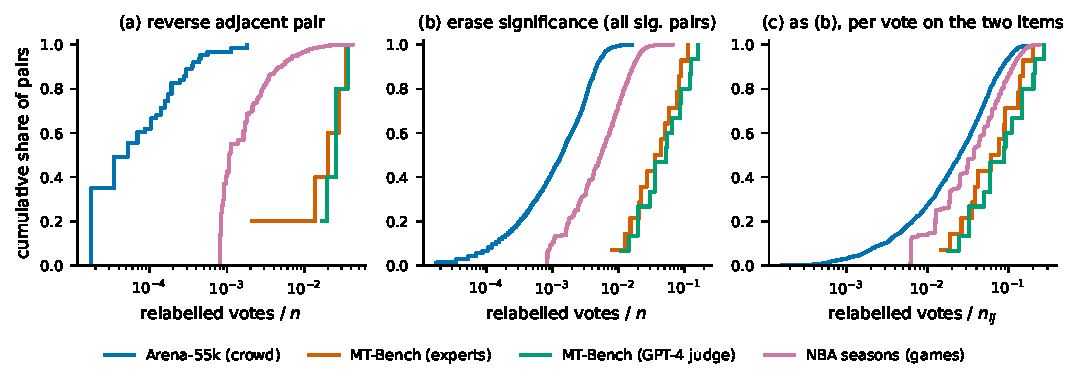
\includegraphics[width=\linewidth]{figs/claims.pdf}
\caption{Cumulative share of pairs that can be changed with a given fraction of votes relabelled. (a) Reversing rank-adjacent pairs; (b) removing significance of all significant pairs; (c) as (b) per vote involving the pair. The curves of (a),(b) are separated by one to two orders of magnitude between boards, those of (c) much less.}\label{fig:claims}
\end{figure}

\subsection{A scale-free summary}\label{sec:scaling}
Figure~\ref{fig:collapse} plots $\kstar/\sqrt{\nij}$ against $z$ for all pairs with finite budgets. Pairs from all four designs fall near one line per edit type, over three orders of magnitude in $\kstar$. Table~\ref{tab:phi} gives the medians. Across the four designs $\hat\varphi$ lies in \Nphimindrop--\Nphimaxdrop{} (delete), \Nphiminrelabel--\Nphimaxrelabel{} (relabel) and \Nphimininsert--\Nphimaxinsert{} (insert); the spread among pairs within a board (10--90\%) is larger than the differences between boards for Arena, MT-Bench and the insertion attack. The largest between-design difference is for relabelling: NBA is higher (\Nphinbarelabel) than the three LLM-evaluation boards (\Nphiarenarelabel, \Nphimthumanrelabel, \NphimtgptFourrelabel); we do not have a verified explanation (candidates: no ties, sparse pairing, the home-field parameter), and the NBA value is stable across seasons (5--95\% of season medians \Nphinbaseasonlorelabel--\Nphinbaseasonhirelabel; only seasons from 1990: \Nphinbamodernrelabel). In log space a regression $\log\kstar=a_{\rm design}+b\log z+c\log\nij$ leaves a residual standard deviation of \Nresidrelabel{} (relabel; \Nresiddrop{} delete, \Nresidinsert{} insert), i.e.\ about 17\% error; but the fitted exponents are $b=$\Nslopezrelabel{} [\Nslopezlorelabel, \Nslopezhirelabel] and $c=$\Nslopenrelabel{} [\Nslopenlorelabel, \Nslopenhirelabel] (cluster bootstrap), not exactly $1$ and $\tfrac12$. We therefore use $\varphi$ as an approximate descriptor, not as a law. Rule of thumb: relabelling about $\kappa\approx\Nkappaminrelabel$--\Nkappamaxrelabel{} votes per unit log-odds gap per vote involving the pair reverses the pair (delete: \Nkappamindrop--\Nkappamaxdrop).

\begin{figure}[t]
\centering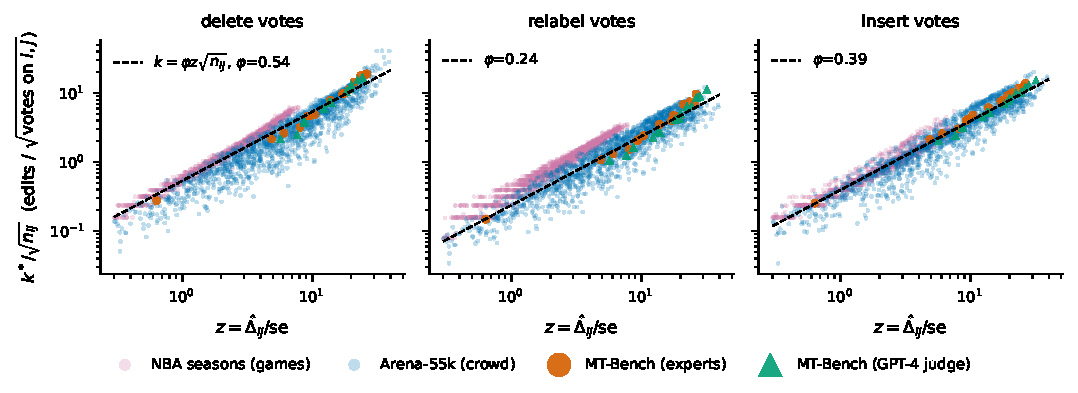
\includegraphics[width=\linewidth]{figs/collapse.pdf}
\caption{Edit budget $\kstar$ scaled by $\sqrt{\nij}$ against the pair's z-score, for the three edit types (log--log; NBA and Arena subsampled to 1,500 pairs for plotting). Dashed: median $\hat\varphi$ over the four designs. Pairs from crowd, expert, LLM-judge and sports data line up along a common slope; the fitted exponents (Sec.~\ref{sec:scaling}) show the line is approximate.}\label{fig:collapse}
\end{figure}

\begin{table}[t]
\caption{Scale-free edit budget for reversing the order of pairs with $z>2$: median $\hat\varphi=\kstar/(z\sqrt{\nij})$ and $\hat\kappa=\kstar/(\Delta_{ij}\nij)$ with 95\% intervals (vote bootstrap for Arena, MT-Bench: 30 replicates; season bootstrap for NBA), and the 10--90\% range of $\varphi$ across pairs of the board. Intervals describe resampling of this board only.}\label{tab:phi}
\centering\scriptsize
\begin{tabular}{llrccc}\toprule
Leaderboard & edit & pairs & $\hat\varphi$ [95\% CI] & pair spread (10--90\%) & $\hat\kappa$ [95\% CI] \\\midrule
Arena-55k (crowd) & delete & 1636 & 0.44 [0.42, 0.46] & 0.23--0.63 & 0.118 [0.111, 0.126] \\
 & relabel & 1636 & 0.24 [0.23, 0.25] & 0.14--0.34 & 0.064 [0.060, 0.068] \\
 & insert & 1636 & 0.37 [0.36, 0.38] & 0.24--0.56 & 0.101 [0.097, 0.105] \\
\addlinespace
MT-Bench (experts) & delete & 14 & 0.57 [0.53, 0.58] & 0.44--0.72 & 0.162 [0.157, 0.166] \\
 & relabel & 14 & 0.24 [0.23, 0.24] & 0.22--0.33 & 0.072 [0.070, 0.074] \\
 & insert & 14 & 0.44 [0.44, 0.46] & 0.43--0.50 & 0.130 [0.126, 0.132] \\
\addlinespace
MT-Bench (GPT-4 judge) & delete & 12 & 0.54 [0.51, 0.57] & 0.38--0.69 & 0.154 [0.149, 0.167] \\
 & relabel & 15 & 0.22 [0.21, 0.23] & 0.18--0.32 & 0.062 [0.061, 0.066] \\
 & insert & 15 & 0.39 [0.38, 0.40] & 0.36--0.46 & 0.112 [0.108, 0.114] \\
\addlinespace
NBA seasons (games) & delete & 9292 & 0.65 [0.64, 0.65] & 0.57--0.76 & 0.144 [0.142, 0.147] \\
 & relabel & 9292 & 0.42 [0.41, 0.42] & 0.35--0.46 & 0.091 [0.089, 0.092] \\
 & insert & 9292 & 0.39 [0.39, 0.40] & 0.35--0.47 & 0.086 [0.084, 0.089] \\
\addlinespace
Arena-140k (crowd, 2025) & delete & 1181 & 0.51 [n/a] & 0.24--0.64 & 0.143 [n/a] \\
 & relabel & 1181 & 0.28 [n/a] & 0.13--0.36 & 0.079 [n/a] \\
 & insert & 1181 & 0.41 [n/a] & 0.24--0.43 & 0.116 [n/a] \\
\bottomrule\end{tabular}

\end{table}

\subsection{Random versus adversarial edits}\label{sec:random}
Figure~\ref{fig:random}a confirms the random-deletion formula within \Nrandvalarena{} (mean absolute difference in the share of adjacent pairs reversed; Arena; \Nrandvalnba{} NBA, \Nrandvalmthuman{} MT-Bench experts). Random deletion of 5\% of the votes leaves rankings close to the original (Kendall $\tau$ with the full ranking \NtauFivearenadrop{} Arena, \NtauFivenbadrop{} NBA, \NtauFivemthumandrop{} MT-Bench experts; random relabelling: \NtauFivearenarelabel, \NtauFivenbarelabel, \NtauFivemthumanrelabel) and reverses only near-ties. A pair with $z=5$ would need $\approx$\NrandneedFive{} of the votes deleted at random for a 5\% reversal probability, but is reversed by adversarial relabelling of a median \Nzfivearena{} (Arena, \Nzfivenarena{} pairs with $4\le z\le6$) to \Nzfivenba{} (NBA, \Nzfivennba{} pairs) of the votes touching it (Fig.~\ref{fig:random}b). Benign noise and adversarial edits of the same size are therefore very different threats.

\begin{figure}[t]
\centering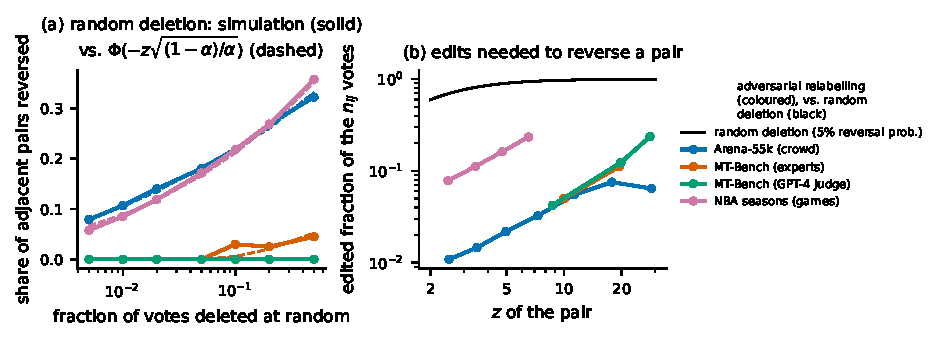
\includegraphics[width=0.92\linewidth]{figs/random.pdf}
\caption{(a) Random vote deletion: simulated share of adjacent pairs reversed (solid) versus $\Phi(-z\sqrt{(1-\alpha)/\alpha})$ computed from the observed $z$ (dashed). (b) Edited fraction of the votes involving a pair needed to reverse it: adversarial relabelling (median per $z$ bin, bins with $\ge3$ pairs) versus random deletion (probability 5\%).}\label{fig:random}
\end{figure}

\subsection{Controls: what changes when the design changes?}\label{sec:control}
\textbf{Same models, different label sources.} Six MT-Bench models also occur in Arena-55k (gpt-4-0314, claude-1, gpt-3.5-turbo-0314, vicuna-13b, alpaca-13b, llama-13b). Table~\ref{tab:matched} compares the Arena crowd votes (1,367 votes among these models) with expert and GPT-4 judgments subsampled to 1,367. The median $z$, the fraction of votes needed and $\hat\varphi$ agree within about 10\% for crowd and experts (relabel: \NAArenarelabelalpha{} vs \NAMTHrelabelalpha{} of the votes, $\hat\varphi$ \NAArenarelabelphi{} vs \NAMTHrelabelphi); the GPT-4 judge gives larger $z$ and so needs more edits (\NAMTGrelabelalpha), with unchanged $\hat\varphi$ (\NAMTGrelabelphi).

\textbf{Same battles, different labellers.} On the same 49,938 battles, LLM-judge labels contain almost no ties and rank models differently from humans (Kendall $\tau$ \NJmistraltau--\NJathenetau{} with the human ranking), yet $\hat\varphi$ (relabel) is \NJathenephi{}, \NJllamaphi{} and \NJmistralphi{} for Athene-70B, Llama-3-8B and Mistral-7B against \NJhumanphi{} for humans (Table~\ref{tab:judges}). Dropping the ties from the human labels moves $\hat\varphi$ to \NJhumannotiesphi, so the near absence of ties accounts for essentially all of the difference. LLM judges yield more separated neighbours (\NJatheneadjsig{} of adjacent pairs significant versus \NJhumanadjsig{} for humans) and higher median $z$.

\textbf{Sample size.} Subsampling Arena (3k--24k votes), MT-Bench (500--2,000) and NBA seasons to 25--50\% shows $\hat\varphi$ nearly constant in $n$ (relabel: Arena \Nscalephiminarenarelabel--\Nscalephimaxarenarelabel, MT-Bench experts \Nscalephiminmthumanrelabel--\Nscalephimaxmthumanrelabel, NBA \Nscalephiminnbarelabel--\Nscalephimaxnbarelabel; appendix Fig.~\ref{fig:control}a). The fraction of votes needed, in contrast, decreases with $n$ (Arena pairs with $z>2$, relabel: \Nscalealphaarenasmall{} at 3k votes to \Nscalealphaarenafull{} at 57k), because larger boards resolve smaller gaps and the pairs entering the $z>2$ set change.

\begin{table}[t]
\caption{Matched control: the same six models rated by Arena crowd votes (all 1,367 available) and by MT-Bench experts and GPT-4 judgments subsampled to $n=1{,}367$. Medians over the 15 pairs; $\pm$: SD over 30 replicates (random subsamples for MT-Bench, vote bootstrap for Arena). $z$ and $\alpha^\ast=\kstar/n$ over all pairs (including capped ones), $\varphi,\kappa$ over pairs with $z>2$.}\label{tab:matched}
\centering\scriptsize
\begin{tabular}{llrrrrr}\toprule
Labels (same 6 models) & edit & $n$ & median $z$ & median $k^*/n$ & $\hat\varphi$ & $\hat\kappa$ \\\midrule
Arena crowd (all available) & delete & 1367 & 9.62$\pm$0.59 & 10.5\%$\pm$1.1\% & 0.51$\pm$0.02 & 0.148$\pm$0.005 \\
 & relabel & 1367 & 9.62$\pm$0.59 & 4.2\%$\pm$0.4\% & 0.23$\pm$0.01 & 0.071$\pm$0.001 \\
 & insert & 1367 & 9.62$\pm$0.59 & 8.3\%$\pm$0.6\% & 0.44$\pm$0.01 & 0.138$\pm$0.002 \\
\addlinespace
MT-Bench experts (subsample) & delete & 1367 & 8.70$\pm$0.81 & 10.2\%$\pm$1.0\% & 0.56$\pm$0.01 & 0.163$\pm$0.003 \\
 & relabel & 1367 & 8.70$\pm$0.81 & 4.4\%$\pm$0.5\% & 0.24$\pm$0.00 & 0.072$\pm$0.001 \\
 & insert & 1367 & 8.70$\pm$0.81 & 8.0\%$\pm$0.7\% & 0.45$\pm$0.01 & 0.130$\pm$0.002 \\
\addlinespace
MT-Bench GPT-4 (subsample) & delete & 1367 & 13.68$\pm$0.34 & 16.7\%$\pm$0.7\% & 0.54$\pm$0.02 & 0.157$\pm$0.005 \\
 & relabel & 1367 & 13.68$\pm$0.34 & 6.5\%$\pm$0.3\% & 0.22$\pm$0.01 & 0.063$\pm$0.001 \\
 & insert & 1367 & 13.68$\pm$0.34 & 11.0\%$\pm$0.4\% & 0.39$\pm$0.01 & 0.112$\pm$0.002 \\
\addlinespace
\bottomrule\end{tabular}

\end{table}

\subsection{Deleting whole questions instead of votes}\label{sec:cluster}
Vote-level edits assume the adversary can pick individual judgments. A more natural curation step removes a whole prompt. On MT-Bench we delete whole questions (all judgments of both turns and all judges of a question) with the same greedy-and-refit search (Table~\ref{tab:cluster}). Reversing a pair with $z>2$ then takes a median \Nclqmth{} of the \Nclnq{} questions (experts), against \Nclvmth{} of the votes at vote level, a ratio of \Nclratiomth, because a question contains judgments in both directions that cannot be separated. The top-1 position (gpt-4 over claude-v1) is reversed by removing \Ncltopmth{} questions (experts) or \Ncltopmtg{} questions (GPT-4 judge). Question-level deletion needs a much larger share of the data; the vote-level numbers are the worst case, not the typical case, for a given leaderboard.

\begin{table}[t]
\caption{Whole-question deletion on MT-Bench: share of the 80 questions that must be removed to reverse a pair with $z>2$, compared with the share of votes at vote level (same pairs; pairs capped at 30\% of votes at vote level are excluded from the ratio, whose range is over pairs; the two medians coincide by chance, the per-pair values differ).}\label{tab:cluster}
\centering\scriptsize
\begin{tabular}{lrrrrr}\toprule
MT-Bench judgments & pairs ($z{>}2$) & questions removed (median share of 80) & votes deleted (median share) & ratio (range) & top-1 reversal (questions) \\\midrule
MT-Bench (experts) & 14 & 68\% & 11.6\% & 5.9 (3.7--8.4) & 11 \\
MT-Bench (GPT-4 judge) & 15 & 68\% & 11.6\% & 5.9 (3.1--11.1) & 30 \\
\bottomrule\end{tabular}

\end{table}

\subsection{Replication on a later snapshot, sessions, and time splits}\label{sec:replic}
On Arena-140k (1{,}378 pairs, same protocol) $\hat\varphi$ is \NphiarenaNewdrop{} (delete), \NphiarenaNewrelabel{} (relabel) and \NphiarenaNewinsert{} (insert), inside the ranges of Table~\ref{tab:phi}; only \NadjsigarenaNew{} of adjacent pairs are significant, and the median adjacent pair is reversed by \NadjkarenaNewrelabel{} relabels or \NadjkarenaNewdrop{} deletions. Evaluation sessions rarely contain several votes (\NarenaNewSessions{} sessions; \NarenaNewMulti{} of the votes sit in multi-vote sessions), and deleting whole sessions needs a median of \Nsessratio{} (range \Nsessratiomin--\Nsessratiomax) times as many sessions as vote-level deletion needs votes, for \Nsesspairs{} random pairs with $z>2$: unlike MT-Bench questions, sessions offer almost no protection. As a natural (non-adversarial) perturbation we compare the first and second half of the votes by timestamp, keeping the \Ntempmodels{} models with at least 300 votes in both halves (\Ntempvotes{} votes): Kendall $\tau$ between the two half-fits is \Ntemptau, against \Nrandtau$\pm$\Nrandtausd{} for 200 random half splits, and \Ntemprev{} of \Nnsigtemp{} pairs significant in the full fit reverse between the time halves, against \Nrandrev$\pm$\Nrandrevsd{} (maximum \Nrandrevmax) under random splits. Within this three-month window, time halves are thus consistent with random ones (a first version without the coverage restriction gave a much lower $\tau$, which we traced to models that enter the arena mid-period and are absent from one half, and discarded).

\subsection{Overtaking cost (rigging-style insertions)}
For the insertion attack, passing a model $r$ places above costs a median of \NovertakekarenarOne{} edits for $r=1$ and \NovertakekarenarFive{} for $r=5$ among Arena models (\NovertakearenarFive{} of the votes for $r=5$), versus \NovertakeknbarFive{} for an NBA season and \NovertakekmthumanrFive{} votes (\NovertakemthumanrFive{}) for MT-Bench ($r=5$; appendix Fig.~\ref{fig:overtake}). These are costs to overtake one specific model with an omniscient attacker and no detection, a lower-effort bound rather than a statement about live systems.

\section{Discussion and limitations}\label{sec:disc}
\textbf{What the evidence supports.} (i) In large leaderboards the ordering of neighbours is not a stable fact: most adjacent pairs are not even significantly different, and a handful of votes (or a fraction of a percent of the votes) reverses them. (ii) The vote fraction needed differs by 1--2 orders of magnitude between designs, but mainly through size and separation: after dividing by $z\sqrt{\nij}$ the designs differ by at most a factor of 1.9 (\Nphimaxrelabel{} vs.\ \Nphiminrelabel{} for relabelling; less for the other edits); in the matched controls label source (crowd, experts, GPT-4) matters little beyond its effect on $z$. (iii) Adversarial edits are orders of magnitude stronger than random ones. \emph{Practical reading:} report tie groups instead of ranks for items within about two standard errors, and judge robustness by $z$ and the number of votes involving the pair, not by the total number of votes. As an illustration of the rule $\kstar\approx\kappa\Delta_{ij}\nij$ (not separately tested): a pair 0.1 log-odds apart (about 17 Elo points) with $\nij=5{,}000$ votes would be reversed by roughly $\Nkappaminrelabel\cdot0.1\cdot5000\approx 31$ to $\Nkappamaxrelabel\cdot0.1\cdot5000\approx 46$ relabelled votes.

\textbf{Conditions and limitations.} \emph{Upper bounds:} $k$ is the size of a verified edit set, not a proven minimum; exhaustive validation covers tiny budgets only, so true minima may be smaller. \emph{Model:} one BT fit with soft ties, not Arena's exact pipeline (no style control, no online Elo); other tie models~\citep{davidson1970,raokupper1967} may give different numbers. \emph{Independence:} edits are single votes and $\mathrm{se}$ treats votes as independent; repeated judgments on the same MT-Bench question, same-user Arena votes, and within-season drift in NBA team strength are ignored, so $z$ overstates the evidence in some cases; edits of whole prompts are examined only for MT-Bench (Sec.~\ref{sec:cluster}) and edits of whole users not at all. \emph{Data:} four leaderboard families, one snapshot each (Arena-55k is a 2024 snapshot of 64 models with a very uneven vote distribution; MT-Bench has 6 models and 15 pairs, so its summaries are noisy; NBA is regular-season outcomes only); results need not hold for other Arena snapshots or for later models. Pair-level samples within a board are not independent and our intervals reflect resampling of one board. \emph{Attacker model:} the adversary knows all votes, may insert votes for any existing pair and outcome, and pays no cost for being detected; real manipulation is harder~\citep{min2025rigging}, so the numbers are best read as a sensitivity bound. Selecting the most influential votes to delete or relabel is an adversarial rule: the numbers bound, but should not be read as a prediction of, the effect of ordinary curation or noise (cf.\ Sec.~\ref{sec:random} and \ref{sec:cluster}). \emph{Unexplained:} NBA's higher $\hat\varphi$ for relabelling and the exact exponents of the scaling relation are described, not explained. \emph{LLM assistance:} the study, code and text were produced by an autonomous LLM agent; see the checklist.

\bibliographystyle{plainnat}
\bibliography{refs}

\appendix
\section{Reproducibility details}
\textbf{Data and checksums.} Arena-55k: \texttt{lmarena-ai/arena-human-preference-55k}, commit \texttt{18c2983\ldots}, \texttt{train.csv} sha256 \texttt{0692154a\ldots}; MT-Bench: \texttt{lmsys/mt\_bench\_human\_judgments}, commit \texttt{f7d2896d\ldots}, human parquet sha256 \texttt{4877bc46\ldots}; NBA: FiveThirtyEight \texttt{nba-elo/nbaallelo.csv}, commit \texttt{4c1ff5e3\ldots}, sha256 \texttt{d46ed354\ldots}; Arena-140k: \texttt{lmarena-ai/arena-human-preference-140k}, commit \texttt{6322995a\ldots} (cc-by-4.0; per-file checksums in \texttt{get\_data.sh}); LLM judges: \texttt{potsawee/chatbot-arena-llm-judges}, commit \texttt{638a7e3b\ldots} (no license stated; used for analysis only, not redistributed). The full environment, commands and a map from each table and figure to its script are in \texttt{README.md} of the supplement; the complete pipeline takes about 45 minutes on 38 CPU cores.

\textbf{Implementation details.} \emph{Votes and edits.} Per configuration $c$ (canonical item pair; for NBA the ordered pair with the home team first, plus the home indicator) we keep counts $N[c,\ell]$, $\ell\in\{0,\tfrac12,1\}$. A unit edit moves one vote between cells: deletion $N[c,\ell]\mathrel{-}=1$; relabelling $N[c,\ell]\mathrel{-}=1,\,N[c,\ell']\mathrel{+}=1$ for any $\ell'\neq\ell$ (ties can become wins and vice versa); insertion $N[c,\ell']\mathrel{+}=1$ with $\ell'\in\{0,1\}$ for any configuration already present in the data. \emph{Greedy search.} In each round the first-order effects of all moves are computed at the current refit (one linear solve), sorted, and moves are taken in order subject to the available counts (relabelling moves from the same cell share its capacity; insertions are unbounded); a batch of $\lceil\hat k/2\rceil$ units is applied, the model is refit by Newton's method with step halving, and the stopping condition is checked on the refit; when it holds, bisection over the prefix of the batch gives the smallest sufficient prefix. Budgets above 30\% of the votes are reported as censored (\Ncensfrac{} of the flip searches). \emph{Data handling.} MT-Bench: both turns and all judges are pooled as independent votes; GPT-4 verdicts ``tie'' and ``tie (inconsistent)'' are both ties. NBA: regular-season games only, one board per season keyed by \texttt{team\_id}, the 19 neutral-site games get home indicator 0. Arena-140k: ``tie'' and ``both bad'' are ties. LLM-judge verdicts are the argmax of the position-averaged probabilities supplied with the dump. Arena-55k votes are used for all 57,477 battles; the single-turn subset (49,938) is used only for the same-battle comparison. Uncertainty for NBA is over seasons, which are not independent samples of one population (rule changes, league size); we treat them as exchangeable replicates of ``a season''.

\begin{figure}[h]
\centering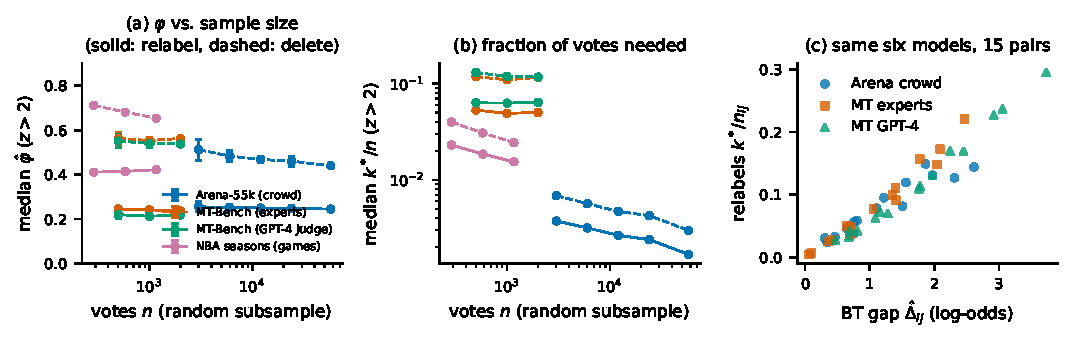
\includegraphics[width=\linewidth]{figs/control.pdf}
\caption{Controls. (a) Median $\hat\varphi$ ($z>2$) versus subsample size, for relabel (solid) and delete (dashed); error bars: SD over replicates. (b) Median fraction of votes needed. (c) The 15 pairs of the six matched models: relabels per vote involving the pair against the BT gap, for crowd, experts and GPT-4 (mean over replicates).}\label{fig:control}
\end{figure}

\begin{figure}[h]
\centering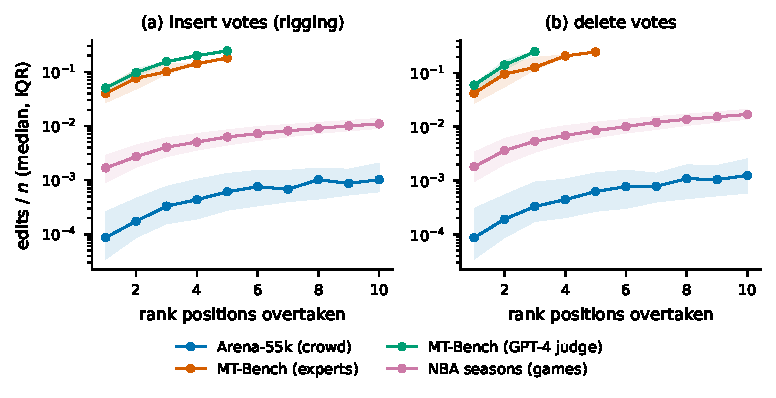
\includegraphics[width=0.85\linewidth]{figs/overtake.pdf}
\caption{Edits (median and inter-quartile range) over $n$ needed to overtake the model $r$ places above, for insertion (a) and deletion (b).}\label{fig:overtake}
\end{figure}

\begin{table}[h]
\caption{Search baselines on pairs with $z>2$ (subsample of pairs: all pairs for MT-Bench; 150 random pairs for Arena; 150 random pairs in each of five NBA seasons). Columns: share of pairs where restricting edits to votes involving $i$ or $j$ gives the same $k$; share where editing only direct $i$--$j$ votes cannot reverse the pair within the 30\% cap; median ratio of random-helpful-edit budget to ours (median of 3 random runs per pair); share of pairs where the random strategy exceeds the cap.}\label{tab:baselines}
\centering\scriptsize
\resizebox{\linewidth}{!}{\begin{tabular}{llrrrrr}\toprule
Leaderboard & edit & pairs & restrict to votes on $i,j$ = full search & only $i$--$j$ votes: infeasible & random helpful edits / ours (median) & random infeasible \\\midrule
Arena-55k (crowd) & delete & 126 & 100\% & 100\% & 2.5 & 0\% \\
 & relabel & 126 & 100\% & 95\% & 2.8 & 0\% \\
 & insert & 126 & 100\% & 42\% & 3.0 & 0\% \\
\addlinespace
MT-Bench (experts) & delete & 14 & 93\% & 86\% & 2.8 & 29\% \\
 & relabel & 14 & 100\% & 43\% & 2.8 & 0\% \\
 & insert & 14 & 100\% & 0\% & 2.9 & 36\% \\
\addlinespace
MT-Bench (GPT-4 judge) & delete & 12 & 100\% & 100\% & 2.1 & 33\% \\
 & relabel & 15 & 100\% & 47\% & 2.5 & 0\% \\
 & insert & 15 & 100\% & 0\% & 5.4 & 47\% \\
\addlinespace
NBA seasons (games) & delete & 349 & 100\% & 100\% & 1.7 & 0\% \\
 & relabel & 349 & 100\% & 98\% & 1.5 & 0\% \\
 & insert & 349 & 100\% & 10\% & 3.5 & 1\% \\
\addlinespace
\bottomrule\end{tabular}
}
\end{table}

\begin{table}[h]
\caption{Same 49,938 Arena battles labelled by humans or LLM judges (relabel edits; all pairs).}\label{tab:judges}
\centering\scriptsize
\resizebox{\linewidth}{!}{\begin{tabular}{lrrrrrrr}\toprule
Labels (same 49,938 battles) & ties & Kendall $\tau$ vs.\ humans & adj.\ pairs $z{>}1.96$ & median $z$ & $\hat\varphi$ (relabel) & $\hat\kappa$ (relabel) & top-1 reversal (relabel) \\\midrule
humans & 31\% & 1.00 & 6\% & 5.7 & 0.24 & 0.064 & 6 \\
humans (no ties) & 0\% & 0.98 & 3\% & 5.4 & 0.28 & 0.057 & 2 \\
Athene-70B & 4\% & 0.79 & 11\% & 9.0 & 0.27 & 0.054 & 5 \\
Llama-3-8B-Inst. & 2\% & 0.71 & 10\% & 8.2 & 0.27 & 0.055 & 4 \\
Mistral-7B-Inst. & 1\% & 0.69 & 8\% & 6.4 & 0.29 & 0.060 & 18 \\
\bottomrule\end{tabular}
}
\end{table}


\newpage
\section*{NeurIPS Paper Checklist}



\begin{enumerate}

\item {\bf Claims}
    \item[] Question: Do the main claims made in the abstract and introduction accurately reflect the paper's contributions and scope?
    \item[] Answer: \answerYes{}
    \item[] Justification: Abstract and introduction state the claims (edit-budget definition, scale-free summaries, comparison across designs, random vs.\ adversarial); they are supported in Sec.~5 and scoped by Sec.~6.
    \item[] Guidelines:
    \begin{itemize}
        \item The answer \answerNA{} means that the abstract and introduction do not include the claims made in the paper.
        \item The abstract and/or introduction should clearly state the claims made, including the contributions made in the paper and important assumptions and limitations. A \answerNo{} or \answerNA{} answer to this question will not be perceived well by the reviewers. 
        \item The claims made should match theoretical and experimental results, and reflect how much the results can be expected to generalize to other settings. 
        \item It is fine to include aspirational goals as motivation as long as it is clear that these goals are not attained by the paper. 
    \end{itemize}

\item {\bf Limitations}
    \item[] Question: Does the paper discuss the limitations of the work performed by the authors?
    \item[] Answer: \answerYes{}
    \item[] Justification: Sec.~6 (conditions and limitations) lists upper-bound searches, the BT/independence assumptions, data snapshots, the omniscient attacker, and the unexplained NBA difference.
    \item[] Guidelines:
    \begin{itemize}
        \item The answer \answerNA{} means that the paper has no limitation while the answer \answerNo{} means that the paper has limitations, but those are not discussed in the paper. 
        \item The authors are encouraged to create a separate ``Limitations'' section in their paper.
        \item The paper should point out any strong assumptions and how robust the results are to violations of these assumptions (e.g., independence assumptions, noiseless settings, model well-specification, asymptotic approximations only holding locally). The authors should reflect on how these assumptions might be violated in practice and what the implications would be.
        \item The authors should reflect on the scope of the claims made, e.g., if the approach was only tested on a few datasets or with a few runs. In general, empirical results often depend on implicit assumptions, which should be articulated.
        \item The authors should reflect on the factors that influence the performance of the approach. For example, a facial recognition algorithm may perform poorly when image resolution is low or images are taken in low lighting. Or a speech-to-text system might not be used reliably to provide closed captions for online lectures because it fails to handle technical jargon.
        \item The authors should discuss the computational efficiency of the proposed algorithms and how they scale with dataset size.
        \item If applicable, the authors should discuss possible limitations of their approach to address problems of privacy and fairness.
        \item While the authors might fear that complete honesty about limitations might be used by reviewers as grounds for rejection, a worse outcome might be that reviewers discover limitations that aren't acknowledged in the paper. The authors should use their best judgment and recognize that individual actions in favor of transparency play an important role in developing norms that preserve the integrity of the community. Reviewers will be specifically instructed to not penalize honesty concerning limitations.
    \end{itemize}

\item {\bf Theory assumptions and proofs}
    \item[] Question: For each theoretical result, does the paper provide the full set of assumptions and a complete (and correct) proof?
    \item[] Answer: \answerNA{}
    \item[] Justification: The paper has no theorems; the heuristic relation for $\varphi$ is explicitly labelled as non-rigorous and the random-deletion formula is checked by simulation (Fig.~3a).
    \item[] Guidelines:
    \begin{itemize}
        \item The answer \answerNA{} means that the paper does not include theoretical results. 
        \item All the theorems, formulas, and proofs in the paper should be numbered and cross-referenced.
        \item All assumptions should be clearly stated or referenced in the statement of any theorems.
        \item The proofs can either appear in the main paper or the supplemental material, but if they appear in the supplemental material, the authors are encouraged to provide a short proof sketch to provide intuition. 
        \item Inversely, any informal proof provided in the core of the paper should be complemented by formal proofs provided in appendix or supplemental material.
        \item Theorems and Lemmas that the proof relies upon should be properly referenced. 
    \end{itemize}

    \item {\bf Experimental result reproducibility}
    \item[] Question: Does the paper fully disclose all the information needed to reproduce the main experimental results of the paper to the extent that it affects the main claims and/or conclusions of the paper (regardless of whether the code and data are provided or not)?
    \item[] Answer: \answerYes{}
    \item[] Justification: Sec.~3--4 and the appendix give the model, edit types, search algorithm, thresholds, caps, data versions and checksums; all runs have fixed seeds and the supplement maps each table and figure to a script.
    \item[] Guidelines:
    \begin{itemize}
        \item The answer \answerNA{} means that the paper does not include experiments.
        \item If the paper includes experiments, a \answerNo{} answer to this question will not be perceived well by the reviewers: Making the paper reproducible is important, regardless of whether the code and data are provided or not.
        \item If the contribution is a dataset and\slash or model, the authors should describe the steps taken to make their results reproducible or verifiable. 
        \item Depending on the contribution, reproducibility can be accomplished in various ways. For example, if the contribution is a novel architecture, describing the architecture fully might suffice, or if the contribution is a specific model and empirical evaluation, it may be necessary to either make it possible for others to replicate the model with the same dataset, or provide access to the model. In general. releasing code and data is often one good way to accomplish this, but reproducibility can also be provided via detailed instructions for how to replicate the results, access to a hosted model (e.g., in the case of a large language model), releasing of a model checkpoint, or other means that are appropriate to the research performed.
        \item While NeurIPS does not require releasing code, the conference does require all submissions to provide some reasonable avenue for reproducibility, which may depend on the nature of the contribution. For example
        \begin{enumerate}
            \item If the contribution is primarily a new algorithm, the paper should make it clear how to reproduce that algorithm.
            \item If the contribution is primarily a new model architecture, the paper should describe the architecture clearly and fully.
            \item If the contribution is a new model (e.g., a large language model), then there should either be a way to access this model for reproducing the results or a way to reproduce the model (e.g., with an open-source dataset or instructions for how to construct the dataset).
            \item We recognize that reproducibility may be tricky in some cases, in which case authors are welcome to describe the particular way they provide for reproducibility. In the case of closed-source models, it may be that access to the model is limited in some way (e.g., to registered users), but it should be possible for other researchers to have some path to reproducing or verifying the results.
        \end{enumerate}
    \end{itemize}


\item {\bf Open access to data and code}
    \item[] Question: Does the paper provide open access to the data and code, with sufficient instructions to faithfully reproduce the main experimental results, as described in supplemental material?
    \item[] Answer: \answerYes{}
    \item[] Justification: All data are public (versions and checksums in the appendix); the supplement contains the full code, \texttt{README.md} with commands and about 45 minutes of expected run time on 38 CPU cores. The code is anonymous.
    \item[] Guidelines:
    \begin{itemize}
        \item The answer \answerNA{} means that paper does not include experiments requiring code.
        \item Please see the NeurIPS code and data submission guidelines (\url{https://neurips.cc/public/guides/CodeSubmissionPolicy}) for more details.
        \item While we encourage the release of code and data, we understand that this might not be possible, so \answerNo{} is an acceptable answer. Papers cannot be rejected simply for not including code, unless this is central to the contribution (e.g., for a new open-source benchmark).
        \item The instructions should contain the exact command and environment needed to run to reproduce the results. See the NeurIPS code and data submission guidelines (\url{https://neurips.cc/public/guides/CodeSubmissionPolicy}) for more details.
        \item The authors should provide instructions on data access and preparation, including how to access the raw data, preprocessed data, intermediate data, and generated data, etc.
        \item The authors should provide scripts to reproduce all experimental results for the new proposed method and baselines. If only a subset of experiments are reproducible, they should state which ones are omitted from the script and why.
        \item At submission time, to preserve anonymity, the authors should release anonymized versions (if applicable).
        \item Providing as much information as possible in supplemental material (appended to the paper) is recommended, but including URLs to data and code is permitted.
    \end{itemize}


\item {\bf Experimental setting/details}
    \item[] Question: Does the paper specify all the training and test details (e.g., data splits, hyperparameters, how they were chosen, type of optimizer) necessary to understand the results?
    \item[] Answer: \answerYes{}
    \item[] Justification: Sec.~4 and the appendix describe protocols, hyper-parameters (ridge $10^{-3}$, batch fraction 0.5, 30\% cap, 1.96 threshold) and how the step fraction was checked (Sec.~5.1); there are no trained models or data splits.
    \item[] Guidelines:
    \begin{itemize}
        \item The answer \answerNA{} means that the paper does not include experiments.
        \item The experimental setting should be presented in the core of the paper to a level of detail that is necessary to appreciate the results and make sense of them.
        \item The full details can be provided either with the code, in appendix, or as supplemental material.
    \end{itemize}

\item {\bf Experiment statistical significance}
    \item[] Question: Does the paper report error bars suitably and correctly defined or other appropriate information about the statistical significance of the experiments?
    \item[] Answer: \answerYes{}
    \item[] Justification: Bootstrap intervals (vote-level, season-level) and replicate SDs are reported for $\hat\varphi,\hat\kappa$ and the controls; they are conditional on the board and do not cover other leaderboards (stated in Sec.~4 and Sec.~6).
    \item[] Guidelines:
    \begin{itemize}
        \item The answer \answerNA{} means that the paper does not include experiments.
        \item The authors should answer \answerYes{} if the results are accompanied by error bars, confidence intervals, or statistical significance tests, at least for the experiments that support the main claims of the paper.
        \item The factors of variability that the error bars are capturing should be clearly stated (for example, train/test split, initialization, random drawing of some parameter, or overall run with given experimental conditions).
        \item The method for calculating the error bars should be explained (closed form formula, call to a library function, bootstrap, etc.)
        \item The assumptions made should be given (e.g., Normally distributed errors).
        \item It should be clear whether the error bar is the standard deviation or the standard error of the mean.
        \item It is OK to report 1-sigma error bars, but one should state it. The authors should preferably report a 2-sigma error bar than state that they have a 96\% CI, if the hypothesis of Normality of errors is not verified.
        \item For asymmetric distributions, the authors should be careful not to show in tables or figures symmetric error bars that would yield results that are out of range (e.g., negative error rates).
        \item If error bars are reported in tables or plots, the authors should explain in the text how they were calculated and reference the corresponding figures or tables in the text.
    \end{itemize}

\item {\bf Experiments compute resources}
    \item[] Question: For each experiment, does the paper provide sufficient information on the computer resources (type of compute workers, memory, time of execution) needed to reproduce the experiments?
    \item[] Answer: \answerYes{}
    \item[] Justification: CPU only; the pipeline takes about 45 minutes on 38 cores and 8\,GB of memory suffice (Sec.~4 and README).
    \item[] Guidelines:
    \begin{itemize}
        \item The answer \answerNA{} means that the paper does not include experiments.
        \item The paper should indicate the type of compute workers CPU or GPU, internal cluster, or cloud provider, including relevant memory and storage.
        \item The paper should provide the amount of compute required for each of the individual experimental runs as well as estimate the total compute. 
        \item The paper should disclose whether the full research project required more compute than the experiments reported in the paper (e.g., preliminary or failed experiments that didn't make it into the paper). 
    \end{itemize}
    
\item {\bf Code of ethics}
    \item[] Question: Does the research conducted in the paper conform, in every respect, with the NeurIPS Code of Ethics \url{https://neurips.cc/public/EthicsGuidelines}?
    \item[] Answer: \answerYes{}
    \item[] Justification: The research uses only public, previously released data and involves no human subjects; we followed the NeurIPS Code of Ethics.
    \item[] Guidelines:
    \begin{itemize}
        \item The answer \answerNA{} means that the authors have not reviewed the NeurIPS Code of Ethics.
        \item If the authors answer \answerNo, they should explain the special circumstances that require a deviation from the Code of Ethics.
        \item The authors should make sure to preserve anonymity (e.g., if there is a special consideration due to laws or regulations in their jurisdiction).
    \end{itemize}


\item {\bf Broader impacts}
    \item[] Question: Does the paper discuss both potential positive societal impacts and negative societal impacts of the work performed?
    \item[] Answer: \answerYes{}
    \item[] Justification: Sec.~6: results help readers judge how much to trust rankings (positive); the same analysis could in principle guide manipulation, but it is an offline model-based bound with an omniscient attacker on public data, and we recommend reporting tie groups.
    \item[] Guidelines:
    \begin{itemize}
        \item The answer \answerNA{} means that there is no societal impact of the work performed.
        \item If the authors answer \answerNA{} or \answerNo, they should explain why their work has no societal impact or why the paper does not address societal impact.
        \item Examples of negative societal impacts include potential malicious or unintended uses (e.g., disinformation, generating fake profiles, surveillance), fairness considerations (e.g., deployment of technologies that could make decisions that unfairly impact specific groups), privacy considerations, and security considerations.
        \item The conference expects that many papers will be foundational research and not tied to particular applications, let alone deployments. However, if there is a direct path to any negative applications, the authors should point it out. For example, it is legitimate to point out that an improvement in the quality of generative models could be used to generate Deepfakes for disinformation. On the other hand, it is not needed to point out that a generic algorithm for optimizing neural networks could enable people to train models that generate Deepfakes faster.
        \item The authors should consider possible harms that could arise when the technology is being used as intended and functioning correctly, harms that could arise when the technology is being used as intended but gives incorrect results, and harms following from (intentional or unintentional) misuse of the technology.
        \item If there are negative societal impacts, the authors could also discuss possible mitigation strategies (e.g., gated release of models, providing defenses in addition to attacks, mechanisms for monitoring misuse, mechanisms to monitor how a system learns from feedback over time, improving the efficiency and accessibility of ML).
    \end{itemize}
    
\item {\bf Safeguards}
    \item[] Question: Does the paper describe safeguards that have been put in place for responsible release of data or models that have a high risk for misuse (e.g., pre-trained language models, image generators, or scraped datasets)?
    \item[] Answer: \answerNA{}
    \item[] Justification: We release no model or data with misuse risk; only analysis code.
    \item[] Guidelines:
    \begin{itemize}
        \item The answer \answerNA{} means that the paper poses no such risks.
        \item Released models that have a high risk for misuse or dual-use should be released with necessary safeguards to allow for controlled use of the model, for example by requiring that users adhere to usage guidelines or restrictions to access the model or implementing safety filters. 
        \item Datasets that have been scraped from the Internet could pose safety risks. The authors should describe how they avoided releasing unsafe images.
        \item We recognize that providing effective safeguards is challenging, and many papers do not require this, but we encourage authors to take this into account and make a best faith effort.
    \end{itemize}

\item {\bf Licenses for existing assets}
    \item[] Question: Are the creators or original owners of assets (e.g., code, data, models), used in the paper, properly credited and are the license and terms of use explicitly mentioned and properly respected?
    \item[] Answer: \answerYes{}
    \item[] Justification: Arena-55k (apache-2.0), MT-Bench judgments (cc-by-4.0) and FiveThirtyEight NBA data (CC-BY-4.0) are cited with versions. The LLM-judge dump used in one experiment states no licence; we used it for analysis only, do not redistribute it, and flag this in the appendix.
    \item[] Guidelines:
    \begin{itemize}
        \item The answer \answerNA{} means that the paper does not use existing assets.
        \item The authors should cite the original paper that produced the code package or dataset.
        \item The authors should state which version of the asset is used and, if possible, include a URL.
        \item The name of the license (e.g., CC-BY 4.0) should be included for each asset.
        \item For scraped data from a particular source (e.g., website), the copyright and terms of service of that source should be provided.
        \item If assets are released, the license, copyright information, and terms of use in the package should be provided. For popular datasets, \url{paperswithcode.com/datasets} has curated licenses for some datasets. Their licensing guide can help determine the license of a dataset.
        \item For existing datasets that are re-packaged, both the original license and the license of the derived asset (if it has changed) should be provided.
        \item If this information is not available online, the authors are encouraged to reach out to the asset's creators.
    \end{itemize}

\item {\bf New assets}
    \item[] Question: Are new assets introduced in the paper well documented and is the documentation provided alongside the assets?
    \item[] Answer: \answerYes{}
    \item[] Justification: No new datasets; the new code is documented in the supplement README.
    \item[] Guidelines:
    \begin{itemize}
        \item The answer \answerNA{} means that the paper does not release new assets.
        \item Researchers should communicate the details of the dataset\slash code\slash model as part of their submissions via structured templates. This includes details about training, license, limitations, etc. 
        \item The paper should discuss whether and how consent was obtained from people whose asset is used.
        \item At submission time, remember to anonymize your assets (if applicable). You can either create an anonymized URL or include an anonymized zip file.
    \end{itemize}

\item {\bf Crowdsourcing and research with human subjects}
    \item[] Question: For crowdsourcing experiments and research with human subjects, does the paper include the full text of instructions given to participants and screenshots, if applicable, as well as details about compensation (if any)? 
    \item[] Answer: \answerNA{}
    \item[] Justification: No crowdsourcing or new human-subject data were collected; we analyse existing public votes.
    \item[] Guidelines:
    \begin{itemize}
        \item The answer \answerNA{} means that the paper does not involve crowdsourcing nor research with human subjects.
        \item Including this information in the supplemental material is fine, but if the main contribution of the paper involves human subjects, then as much detail as possible should be included in the main paper. 
        \item According to the NeurIPS Code of Ethics, workers involved in data collection, curation, or other labor should be paid at least the minimum wage in the country of the data collector. 
    \end{itemize}

\item {\bf Institutional review board (IRB) approvals or equivalent for research with human subjects}
    \item[] Question: Does the paper describe potential risks incurred by study participants, whether such risks were disclosed to the subjects, and whether Institutional Review Board (IRB) approvals (or an equivalent approval/review based on the requirements of your country or institution) were obtained?
    \item[] Answer: \answerNA{}
    \item[] Justification: No human-subject research was conducted.
    \item[] Guidelines:
    \begin{itemize}
        \item The answer \answerNA{} means that the paper does not involve crowdsourcing nor research with human subjects.
        \item Depending on the country in which research is conducted, IRB approval (or equivalent) may be required for any human subjects research. If you obtained IRB approval, you should clearly state this in the paper. 
        \item We recognize that the procedures for this may vary significantly between institutions and locations, and we expect authors to adhere to the NeurIPS Code of Ethics and the guidelines for their institution. 
        \item For initial submissions, do not include any information that would break anonymity (if applicable), such as the institution conducting the review.
    \end{itemize}

\item {\bf Declaration of LLM usage}
    \item[] Question: Does the paper describe the usage of LLMs if it is an important, original, or non-standard component of the core methods in this research? Note that if the LLM is used only for writing, editing, or formatting purposes and does \emph{not} impact the core methodology, scientific rigor, or originality of the research, declaration is not required.
    %this research? 
    \item[] Answer: \answerYes{}
    \item[] Justification: The study was run by an autonomous LLM agent (Claude) that wrote the code, ran the experiments and drafted the text, working from the public task description; no LLM is part of the studied methods, and the LLM judges in Sec.~5.5 are public pre-computed verdicts from a third-party data release. Every number in the paper is generated by the supplied code.
    \item[] Guidelines:
    \begin{itemize}
        \item The answer \answerNA{} means that the core method development in this research does not involve LLMs as any important, original, or non-standard components.
        \item Please refer to our LLM policy in the NeurIPS handbook for what should or should not be described.
    \end{itemize}

\end{enumerate}
\end{document}
